\documentclass[12pt]{article}
% adjust style for page
\usepackage{fancyhdr}
% adjust the gap between content and margins of pages 
\usepackage{geometry}
% import images
\usepackage{graphicx} 
% tweak math elements
\usepackage{amsmath}
% import other .tex files into the main .tex
\usepackage{import}
% for simulating model content
\usepackage{lipsum}
% for hyper link that connects to other URL
\usepackage{hyperref}
% for tables having specific width
\usepackage{tabularx} 
% together used with "tabularx" package
\usepackage{booktabs}
% control position of elements precisely
\usepackage{float}
% control the caption element for table and figure
\usepackage{caption}
% for some math symbols and format
\usepackage{amsmath} % for 'cases' environment
% To manage footnotes in tables
\usepackage{threeparttable}  
% i forget the function of this one, GPT told me to include it :) 
\usepackage{babel}
% for multirows
\usepackage{multirow}
% for biblatex
% \usepackage[backend=biber]{biblatex}
% for hyper link
\usepackage{hyperref}

\newenvironment{myfigure}[3] % width, path, caption
{
    \begin{figure}[htbp]
        \centering
        \includegraphics[width=#1\textwidth]{#2}
        \caption{#3}
}
{
    \end{figure}
}
\usepackage{hyperref}
\usepackage{xcolor}


\title{
This is title
}

\author{Feng Gu(T00751197), author 2 and author 3}
% \date{\today}

\begin{document}
\maketitle

\begin{center}
    \textbf{\large Abstract}
    Here to attach abstract.
\end{center}

\section{Introduction}
In this project, we aim to develop regression models to predict the energy consumption
 of appliances in a low-energy building. The dataset includes various environmental and 
 meteorological features, such as indoor temperature, humidity, and outdoor conditions. 
We explore both linear and non-linear models, focusing on feature selection, model evaluation,
and hyperparameter tuning to achieve accurate and interpretable predictions. 
The analysis highlights the trade-offs between model com-plexity and performance.

\section{Data srouce and description}

The Appliances Energy Prediction dataset comprises experimental data collected over approximately 4.5 months
at 10-minute intervals. It is designed for regression analysis, aiming to model the energy consumption
of appliances in a low-energy building. The dataset includes 19,735 instances, each characterized by
28 features encompassing indoor environmental conditions, energy usage, and local meteorological data.
Notably, the dataset contains no missing values.

To access the dataset, please visit the UCI Machine Learning Repository at the following link:
\href{https://archive.ics.uci.edu/dataset/374/appliances+energy+prediction}{\textit{Data set: Appliances Energy Prediction}}

\subsection{Variable information}
Key features in the dataset are shown in Table \ref{tab:energy_appliances}. 
The target variable is the energy consumption of appliances, 
while other features include temperature and humidity readings from various rooms, 
outdoor temperature, pressure, humidity, wind speed, visibility, and dew point. 
Two random variables (RV\_1 and RV\_2) are also included to account for potential noise in the data.
The dataset also includes a time variable indicating the number of seconds since midnight and 
the date in the format \%Y-\%M-\%D \%H:\%M.

\begin{table}[!h]
    \centering
    \caption{Data Variables in the Energy Appliances Data Set}
    \begin{tabular}{l l c}
        \toprule
        \textbf{Data Variables} & \textbf{Units} & \textbf{Number of Features} \\
        \midrule
        Appliances energy consumption & Wh & 1 \\
        Light energy consumption & Wh & 2 \\
        $T_i$: Temperature in room $i$ & °C & 3-21 \\
        $RH_i$: Humidity in room $i$ & \% & 4-20 \\
        Temperature outside & °C & 21 \\
        Pressure  & mm Hg & 22 \\
        Humidity outside & \% & 23 \\
        Windspeed & m/s & 24 \\
        Visibility & km & 25 \\
        Dew point & °C & 26 \\
        Random Variable 1 (RV\_1) & - & 27 \\
        Random Variable 2 (RV\_2) & - & 28 \\
        Number of seconds from midnight  & s & 29 \\
        date & \%Y-\%M-\%D \%H:\%M & 30 \\
        \bottomrule
    \end{tabular}
    \label{tab:energy_appliances}
\end{table}

% waiting to be refined
However, time series related problems are not the focus of this project, the time variable will \textbf{only be used to 
create dummy variables} for the month status. \textbf{The potential autocorrelation in the data will be ignored}.

\section{Data preprocessing}
\subsection{Create dummy variables}
For the month status, we create dummy variables for each month by extracting the month from the time variable.
To aviod multicollinearity, we set January as the reference month and drop the corresponding dummy variable.

\subsection{Detect and remove outliers}
We calculated the skewness of each feature in the dataset to detect outliers.

The skewness $\gamma_1$ of a random variable $X$ is the third \textbf{{standardized moment}} 
$\tilde{\mu}_3$ \footnote{Reference from 'Wikipedia' about 'Skewness'.}

\[
\gamma_1 = \tilde{\mu}_3 = E \left[ \left( \frac{X - \mu}{\sigma} \right)^3 \right] = \frac{\mu_3}{\sigma^3} = \frac{E[(X - \mu)^3]}{\left(E[(X - \mu)^2]\right)^{3/2}} = \frac{\kappa_3}{\kappa_2^{3/2}}.
\]

To features that have skewness great than 1(there are only two features meeting this condition),
we filter out the outliers by mannually choosing the threshold value - 95\% quantile. After checking the relationship between
the outliers and target values, we found that the outliers are not related to the target values, so we remove them from the dataset. 
The distribution plot of the features before and after removing the outliers is shown in Figure \ref{fig:skewness}.

After removing the outliers, we left with 19,647 instances and 28 features.

\subsection{Feature selection}
We used Lasso regression to select the most important features from the dataset, and use the selected features to build the model.
The optimization problem for Lasso regression can be formulated as:

\[
\hat{\beta} = \arg\min_{\beta} \left\{ \frac{1}{n} \sum_{i=1}^n \left( y_i - \mathbf{x}_i^\top \beta \right)^2 + \lambda \sum_{j=1}^p |\beta_j| \right\}
\]

The reason we chose lasso instead of ridge is that the lasso penalty, \( \lambda \sum_{j=1}^p |\beta_j| \), encourages sparsity in the coefficients, 
which drop some of coefficients to zero when some features are highly correlated. However, ridge regression will not 
drop the highly correlated features, but will give them similar coefficients, which does not help to reduce the model complexity.

By setting different values of \(\lambda\), we can get different number of features, the value of \(\lambda\) is chosen by cross-validation using 
the adjusted \(R^2\) criterion. 
\textbf{We modulized this process in to a function that will be envoked in the later model building process.} 
A demonstration of the feature selection process is shown in Figure \ref{fig:lasso}.

\section{Polynomial Linear regression with LASSO-based Feature Selection}

\subsection{Search for the best model}

In this analysis, we evaluated the performance of polynomial regression models of degree 1 and 2 using
 a subset of predictors selected through LASSO regression. The feature selection process was based on a
  range of LASSO regularization values ($\lambda$), specifically $\lambda \in \{0.001, 0.01, 0.05, 0.1, 0.15\}$.
   For each $\lambda$ value, we identified the non-zero coefficient predictors selected by the LASSO model 
   and used them as input features in subsequent regression analysis.

All selected predictors were standardized using the \texttt{StandardScaler} to ensure zero mean 
and unit variance. The target variable (\texttt{Appliances}) was also standardized to facilitate proper 
comparison of errors across different model configurations. The dataset was then split into equal halves, 
with 80\% used for training and 20\% used for testing. A fixed random seed was used to ensure reproducibility of results.

For each combination of $\lambda$ and polynomial degree (1 for linear and 2 for quadratic regression), 
we trained a regression pipeline consisting of a \texttt{PolynomialFeatures} transformer followed by a 
standard \texttt{LinearRegression} model. The models were evaluated on both training and testing data using
a comprehensive set of performance metrics.

\begin{table}[!h]
    \centering
    \caption{Polynomial Regression Model Evaluation Metrics}
    \label{tab:metrics}
    \begin{tabular}{ccccccccc}
    \toprule
    \textbf{$\lambda$} & \textbf{Degree} & \textbf{$p$} & \textbf{MSE} & \textbf{MAE} & \textbf{train $\bar R^2$} & \textbf{test $\bar R^2$} & \textbf{LogLikeli} & \textbf{AIC} \\
    \midrule
    \multirow{2}{*}{0.0010} & 1 & 30 & 0.7171 & 0.5932 & 0.2873 & 0.2648 & -19688.08 & 39438.16 \\
                            & 2 & 58 & 0.5004 & 0.5031 & 0.5027 & 0.4348 & -16859.91 & 34711.82 \\
                            \hline
    \multirow{2}{*}{0.0100} & 1 & 20 & 0.7279 & 0.5955 & 0.2774 & 0.2539 & -19806.02 & 39654.04 \\
                            & 2 & 38 & 0.5827 & 0.5343 & 0.4216 & 0.3861 & -18057.00 & 36575.99 \\
                            \hline
    \multirow{2}{*}{0.0500} & 1 & 12 & 0.7767 & 0.6250 & 0.2298 & 0.2102 & -20315.69 & 40657.38 \\
                            & 2 & 22 & 0.6790 & 0.5759 & 0.3267 & 0.2995 & -19259.59 & 38701.19 \\
                            \hline
    \multirow{2}{*}{0.1000} & 1 & 10 & 0.7965 & 0.6333 & 0.2104 & 0.1901 & -20512.99 & 41047.98 \\
                            & 2 & 18 & 0.7062 & 0.5925 & 0.3000 & 0.2818 & -19567.34 & 39266.68 \\
                            \hline
    \multirow{2}{*}{0.1500} & 1 & 7 & 0.8493 & 0.6531 & 0.1583 & 0.1445 & -21018.23 & 42052.45 \\
                            & 2 & 12 & 0.8284 & 0.6477 & 0.1791 & 0.1619 & -20822.10 & 41716.20 \\   
    \bottomrule
    \end{tabular}
\end{table}

\subsection{Model evaluation and residual analysis}
The metrics included the loglikelihood, AIC, Mean Squared Error (MSE) and Mean Absolute Error (MAE) on the training set, 
as well as the adjusted $R^2$ scores on both the training and testing sets.

Based on the performance metrics presented in Table~\ref{tab:metrics}, 
the best model appears to be the polynomial regression of degree 2 under 
the LASSO regularization parameter $\lambda = 0.001$. This model achieves 
the lowest Mean Squared Error (MSE = 0.5004) and the lowest Mean Absolute Error 
(MAE = 0.5031), along with the highest adjusted $R^2$ on both the training set 
($\bar{R}^2 = 0.5027$) and the test set ($\bar{R}^2 = 0.4348$). 

Furthermore, this model provides the highest log-likelihood and the lowest Akaike Information
Criterion (AIC = 34711.82), which jointly indicate a better fit to the data while appropriately
penalizing model complexity. Taken together, these metrics suggest that the $\lambda = 0.001$,
degree 2 model balances bias and variance most effectively and is the most suitable model 
among the candidates evaluated.

\begin{figure}[!h]
    \centering
    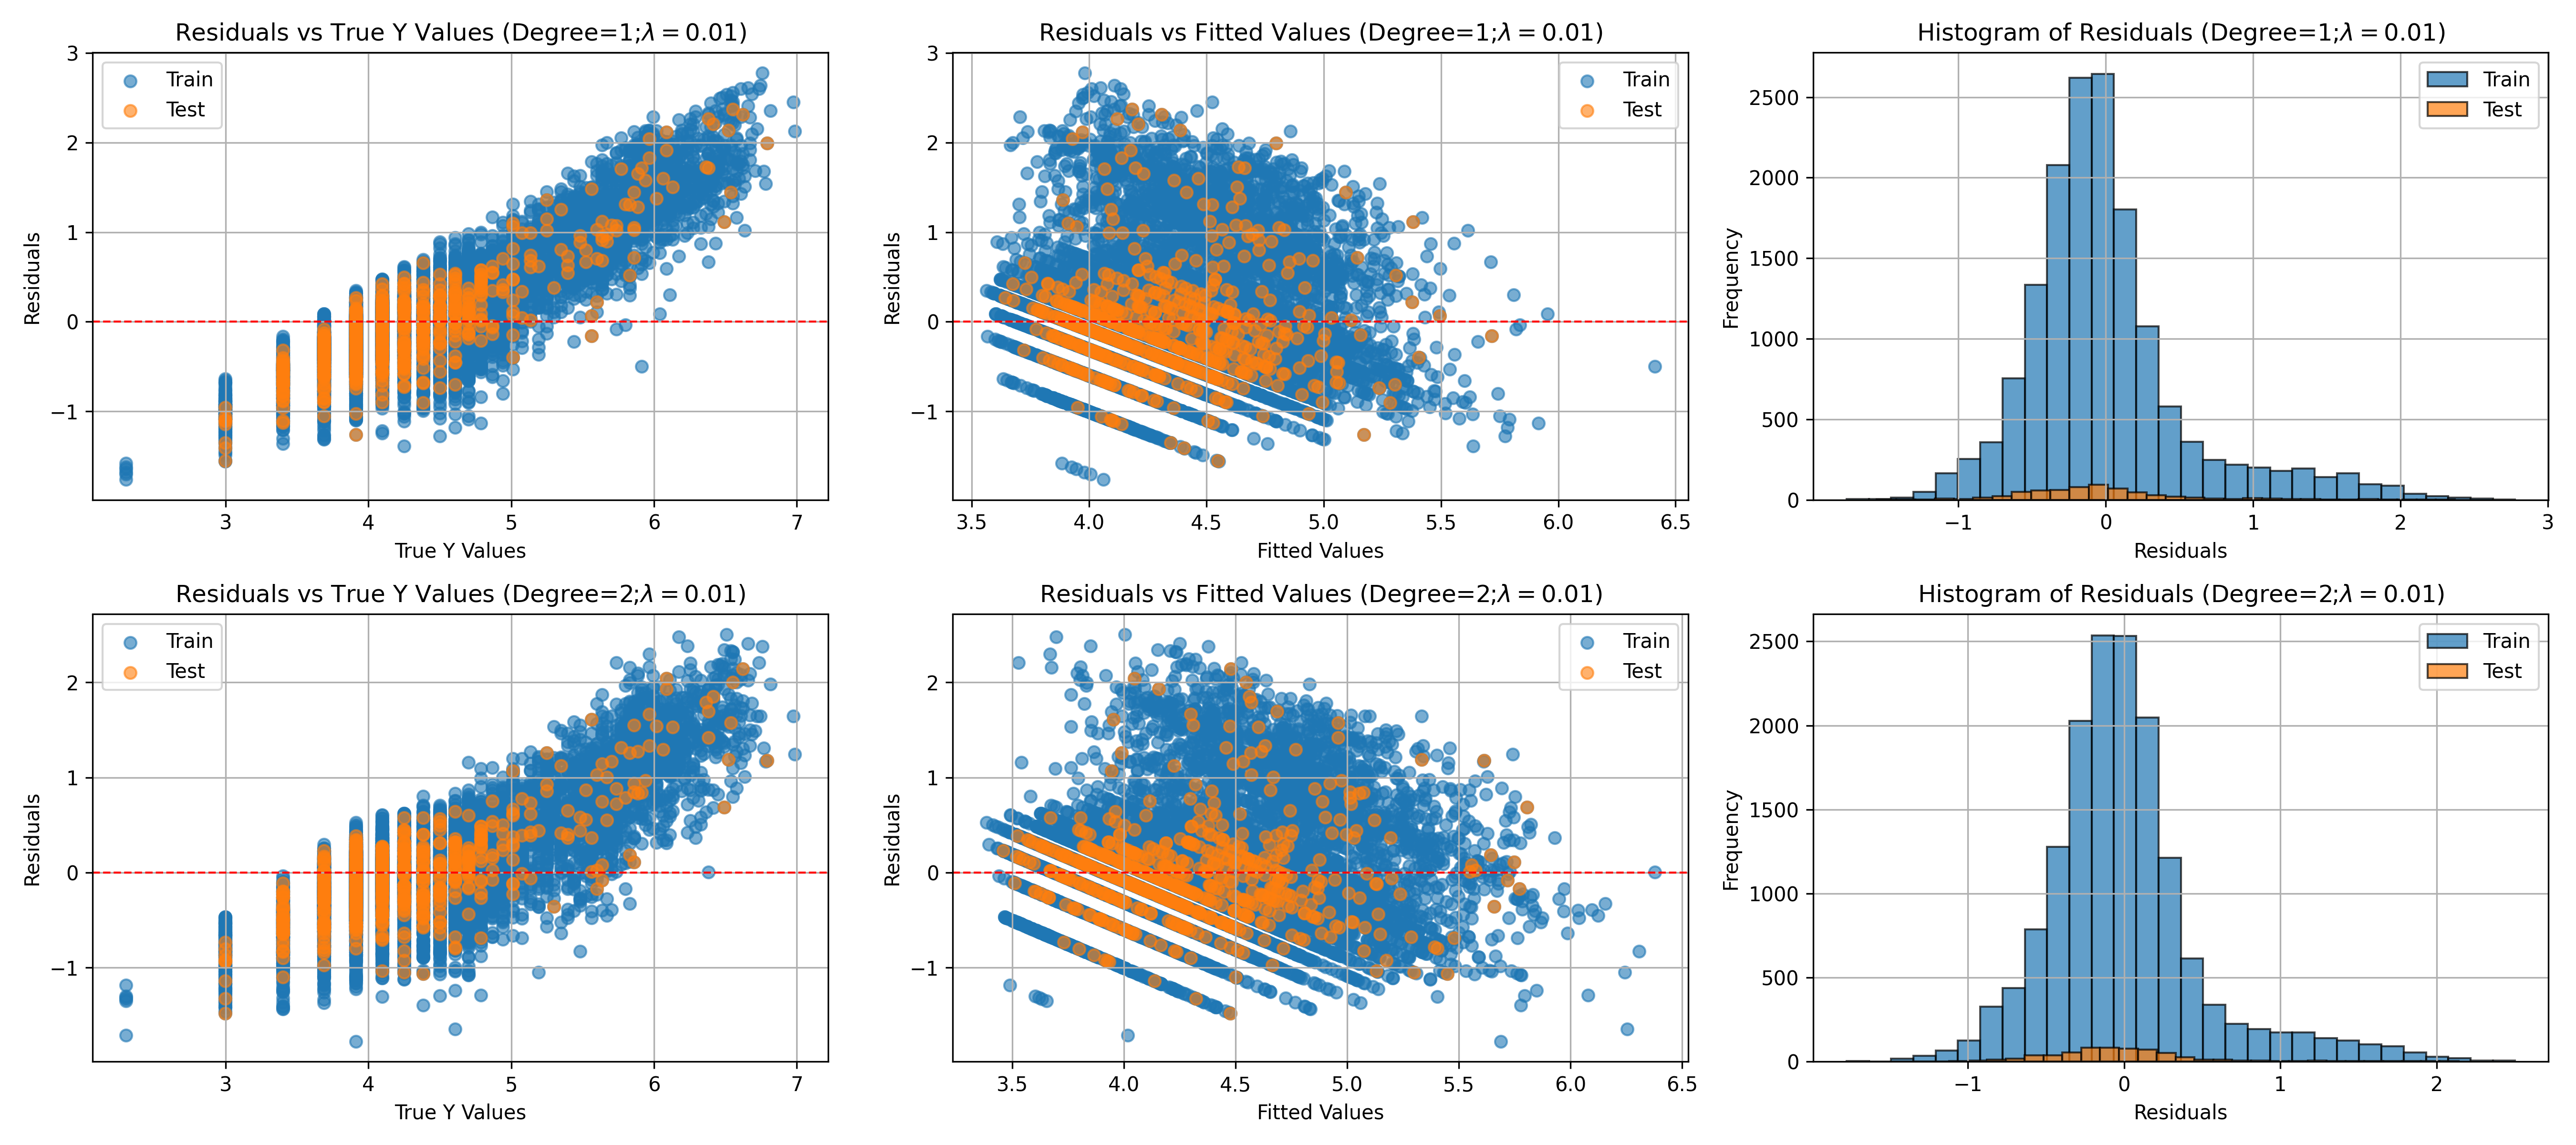
\includegraphics[width=1\textwidth]{../results/linear_residuals_analysis.png}
    \caption{Residual analysis of the linear regression model}
    \label{fig:linear_residuals}
\end{figure}


Figure~\ref{fig:linear_residuals} shows residual diagnostics for polynomial 
regression models of degree 1 and 2 under $\lambda = 0.01$.
 Both models have residuals centered around zero, indicating unbiased predictions.
  However, the degree 2 model exhibits a more symmetric and tighter residual distribution,
   closer to normality, compared to the slightly right-skewed residuals of the degree 1 model.

The residuals vs. fitted values plot for the degree 1 model shows a fan-shaped pattern, 
suggesting heteroscedasticity and underfitting. In contrast, the degree 2 model displays more 
evenly spread residuals, indicating better fit and variance stability.
 Residuals vs. true $y$ plots also show tighter clustering for the degree 2 model, confirming its superior performance.

Table~\ref{tab:linear_regression} presents OLS regression results for \texttt{Appliances},
 with an $R^2$ of 0.268, explaining 26.8\% of the variance. The F-statistic is significant 
 ($p < 0.001$), indicating the model's overall significance. Most predictors are significant at 
 the 1\% level, except \textbf{RH\_3} ($p = 0.275$) and \textbf{Visibility} ($p = 0.239$), which may be excluded for simplicity.

Residual diagnostics reveal non-normality (skewness = 1.309, kurtosis = 5.736) and a 
high condition number ($1.02 \times 10^5$), suggesting potential multicollinearity and the need for further investigation.

\section{Kernel regression}
Parametric regression might not be the best choice for this dataset, 
therefore we also non-parametric method - kernel regression.

\subsection{Choice of kernel}
The kernel regression function is defined as:

\[
\hat{f}(x) = \frac{\sum_{i=1}^n K\left(\frac{x - x_i}{h}\right) y_i}{\sum_{i=1}^n K\left(\frac{x - x_i}{h}\right)},
\]

where \( K(\cdot) \) is the kernel function, \( h \) is the bandwidth parameter, \( x_i \) are the input data points, and \( y_i \) are the corresponding output values.

In our report, we use a commonly used kernel that is the Radial Basis Function (RBF) kernel, which is defined as:

\[
K(x, x') = \exp\left(-\frac{\|x - x'\|^2}{2\sigma^2}\right),
\]

where \( \|x - x'\| \) is the Euclidean distance between \( x \) and \( x' \), and \( \sigma \) is a parameter that controls the width of the kernel.

\subsection{Hyperparameter Tuning in Kernel Ridge Regression}

In the KRR
\footnote{Kernel Ridge Regression} 
with RBF kernel framework, two hyperpa-rameters: 
\(\alpha\) and 
\(\gamma\)—play crucial roles in controlling model complexity and smoothness. 
The regularization parameter \(\alpha > 0\) penalizes the magnitude of the model
coefficients, effectively shrinking them towards zero to prevent overfitting. 
Larger values of \(\alpha\) impose stronger regularization, leading to simpler
models with potentially higher bias but lower variance\footnote{We used Lasso regression to select features before we trained kernel model, 
here we used \(L_2\) penalty in kernel regression again to avoid overfitting upon this sub-data set.}.
On the other hand, \(\gamma\)
is a shape parameter specific to the radial basis function (RBF) kernel. It controls
the width of the Gaussian kernel, with smaller values producing smoother functions
and larger values allowing the model to adapt more closely to the training data.

To select optimal values for these hyperparameters, we performed an exhaustive grid search over a predefined parameter space:
\[
\alpha \in \{0.01, 0.1, 0.5, 1.0\}, \quad \gamma \in \{0.001, 0.01, 0.05, 0.1\}.
\]
For each pair \((\alpha, \gamma)\), we trained a KRR model using standardized predictors
and evaluated it on both training and test sets. Model performance was assessed using 
multiple metrics: Mean Squared Error (MSE), Mean Absolute Error (MAE), and the coefficient 
of determination \(R^2\). By systematically comparing the results across different configurations, 
we identified the hyperparameter combination that provided the best trade-off between underfitting and overfitting.

\subsection{Kernel Ridge Regression Results with RBF Kernel}

Table~\ref{tab:best_kernel_models} presents the best RBF kernel regression
results across different feature sets selected by Lasso with varying $\lambda$. 
For each subset, we tuned $\alpha$ (regularization strength) and $\gamma$ (kernel width) to minimize prediction error.

\begin{table}[!h]
    \centering
    \caption{Best pamameters of KRR under different feature selection}
    \label{tab:best_kernel_models}
    \begin{tabular}{ccccccc}
    \toprule
    \textbf{$\lambda$} & \textbf{$\alpha$} & \textbf{$\gamma$} & \textbf{Train MSE} & \textbf{Test MSE} & \textbf{Train $R^2$} & \textbf{Test $R^2$} \\
    \midrule
    0.0010 & 0.01 & 0.01 & 0.1456 & 0.2512 & 0.6714 & 0.3622 \\
    0.0050 & 0.01 & 0.01 & 0.1755 & 0.2574 & 0.5794 & 0.3581 \\
    0.0100 & 0.01 & 0.01 & 0.1910 & 0.2474 & 0.5696 & 0.3495 \\
    0.0500 & 0.10 & 0.05 & 0.2147 & 0.2931 & 0.4706 & 0.3275 \\
    \bottomrule
    \end{tabular}
\end{table}

Eventhough the optimal performance was achieved when $\lambda = 0.001$, $\alpha = 0.01$, and $\gamma = 0.01$,
the model still performed well with $\lambda = 0.01$, $\alpha = 0.01$, and $\gamma = 0.01$.
The difference between the two models is marginal, but the features selected under $\lambda = 0.01$ is 20, which is 
significanly less than the 30 features selected under $\lambda = 0.001$.
This indicates that the model is less complex and more interpretable, while still maintaining good predictive performance, and 
we choose this model as the final model.

\subsection{Model evaluation and residual analysis}

\begin{figure}[!h]
    \centering
    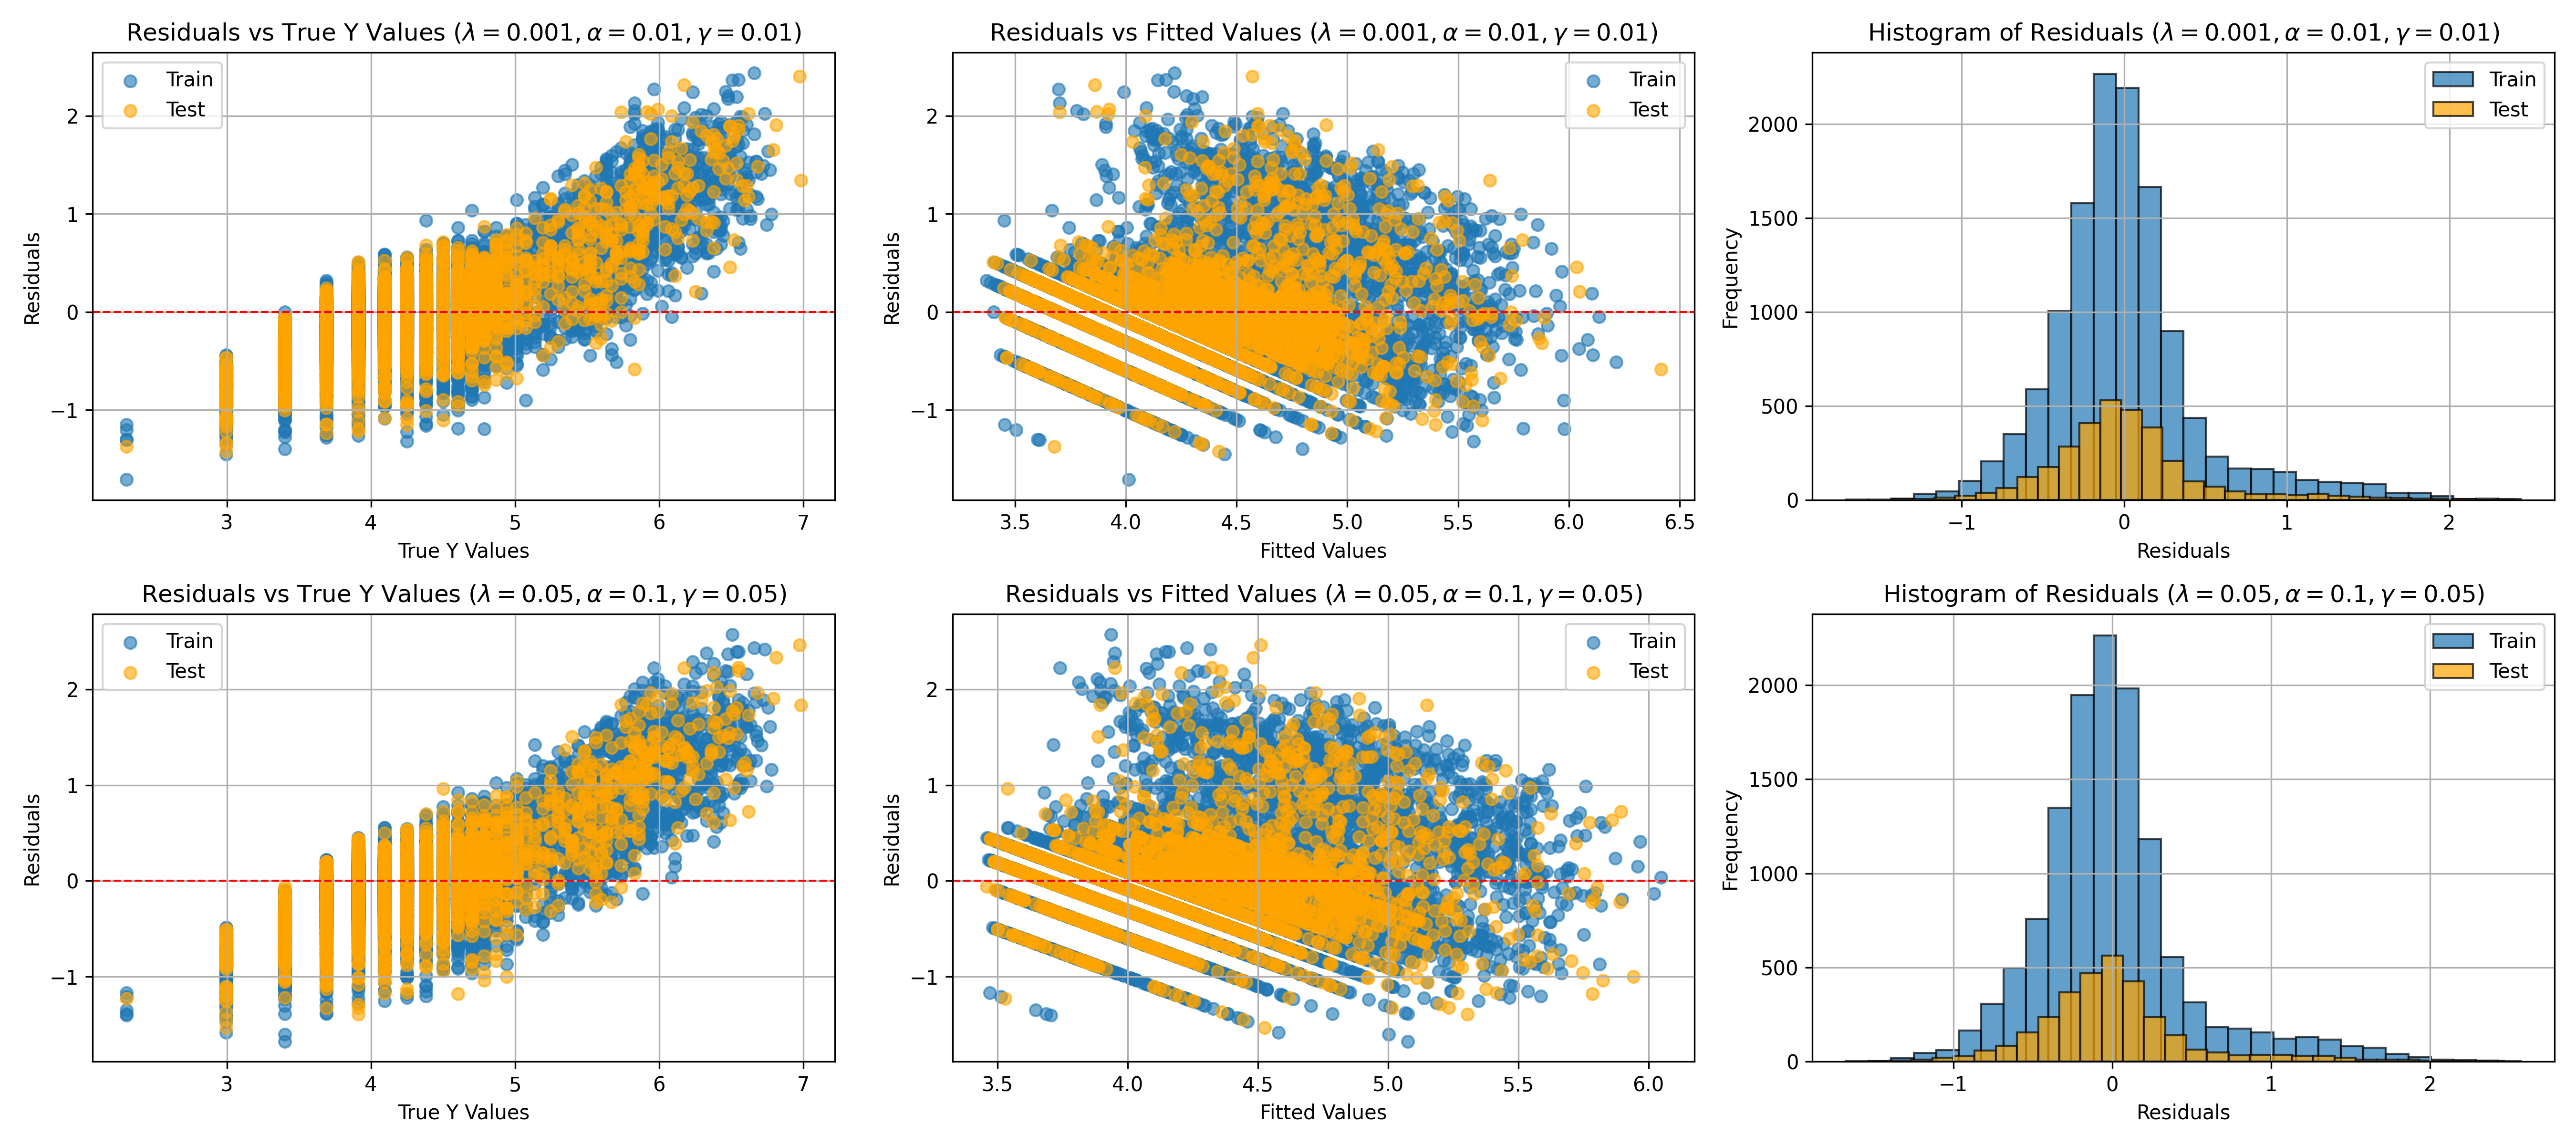
\includegraphics[width=1\textwidth]{../results/kernel_residuals_analysis.png}
    \caption{Residual analysis of the kernel regression model}
    \label{fig:kernel_residuals}
\end{figure}

Figure~\ref{fig:kernel_residuals} presents the residual analysis for two kernel regression models. 
The first row corresponds to the model with lower complexity or less regularization, 
while the second row shows a more regularized model. 

In both cases, the residuals appear to be centered around zero, indicating that the models
 are generally unbiased. However, the residuals in the first model exhibit more visible patterns 
 and heteroscedasticity, especially in the \textit{residuals vs fitted values} plot, suggesting 
 that the model may slightly underfit or fail to capture some nonlinear structures.

The second model shows a more randomly scattered residual pattern, especially in the 
\textit{residuals vs fitted} plot, which is desirable and indicates better model specification. 
The histograms of residuals for both training and test sets in the second model are more symmetric 
and closer to a normal distribution compared to the first model, supporting the conclusion that
 the second model generalizes slightly better.

\section{Conlcustion}
In conclusion, this project explored both linear and kernel regression
 models to predict the energy consumption of appliances in a low-energy building. 
The linear regression model, particularly the polynomial regression of degree 2 with LASSO-based feature selection,
demonstrated reasonable performance with an adjusted $R^2$ of 0.4348 on the test set. 
However, this model uses 58 features, which may lead to overfitting and reduced interpretability.


On the other hand, the kernel regression model with an RBF kernel performed well, 
achieving test $R^2$ of 0.3622 and 0.3495 using only 30 and 12 features, under optimal hyperparameter settings.

While the linear model offers higher test $R^2$ and interpretability,
it struggled to capture the nonlinear relationships in the data and needed too many features.

In contrast,
the kernel regression model, though hard to interprate, provided better flexibility
and predictive accuracy by using significantly less features.
Ultimately, the kernel regression model was selected as the final
model due to its superior performance and ability to generalize better to unseen data.

\section{Future work}
In future work, the following improvements can be made:

\begin{itemize}
    \item \textbf{Efficient Hyperparameter Search:} 
    Replace exhaustive grid search with advanced techniques like random search,
     Bayesian optimization, or genetic algorithms. These methods can significantly 
     reduce computation time while exploring the hyperparameter space more effectively.

    \item \textbf{Modularized Codebase:} 
    Further modularize the code by creating separate, reusable functions or
     classes for preprocessing, feature selection, model training, and evaluation.
      This will enhance code readability, maintainability, and scalability for future extensions.
\end{itemize}

\section{References}

\begin{thebibliography}{99}

    \bibitem{vanderPlas2022}
    Jake VanderPlas.
    \textit{Python Data Science Handbook}, 2nd edition.
    O'Reilly Media, 2022. ISBN: 9781098121198. \textit{Anna’s Archive}.
    
    \bibitem{mckinney2017}
    Wes McKinney.
    \textit{Python for Data Analysis}, 2nd edition.
    O'Reilly Media, 2017. ISBN: 9781491957660.
    
    \bibitem{seabold2010statsmodels}
    Skipper Seabold and Josef Perktold.
    Statsmodels: Econometric and Statistical Modeling with Python.
    In \textit{9th Python in Science Conference}, 2010.
    
    \bibitem{sklearn_api}
    Lars Buitinck, Gilles Louppe, etc.\\
    \textit{API design for machine learning software: experiences from the scikit-learn project}.\\
    In \textit{ECML PKDD Workshop: Languages for Data Mining and Machine Learning}, 2013, pages 108--122.
    
    \end{thebibliography}

\section{Appendix}

\subsection{Figures}
\begin{figure}[!h]
    \centering
    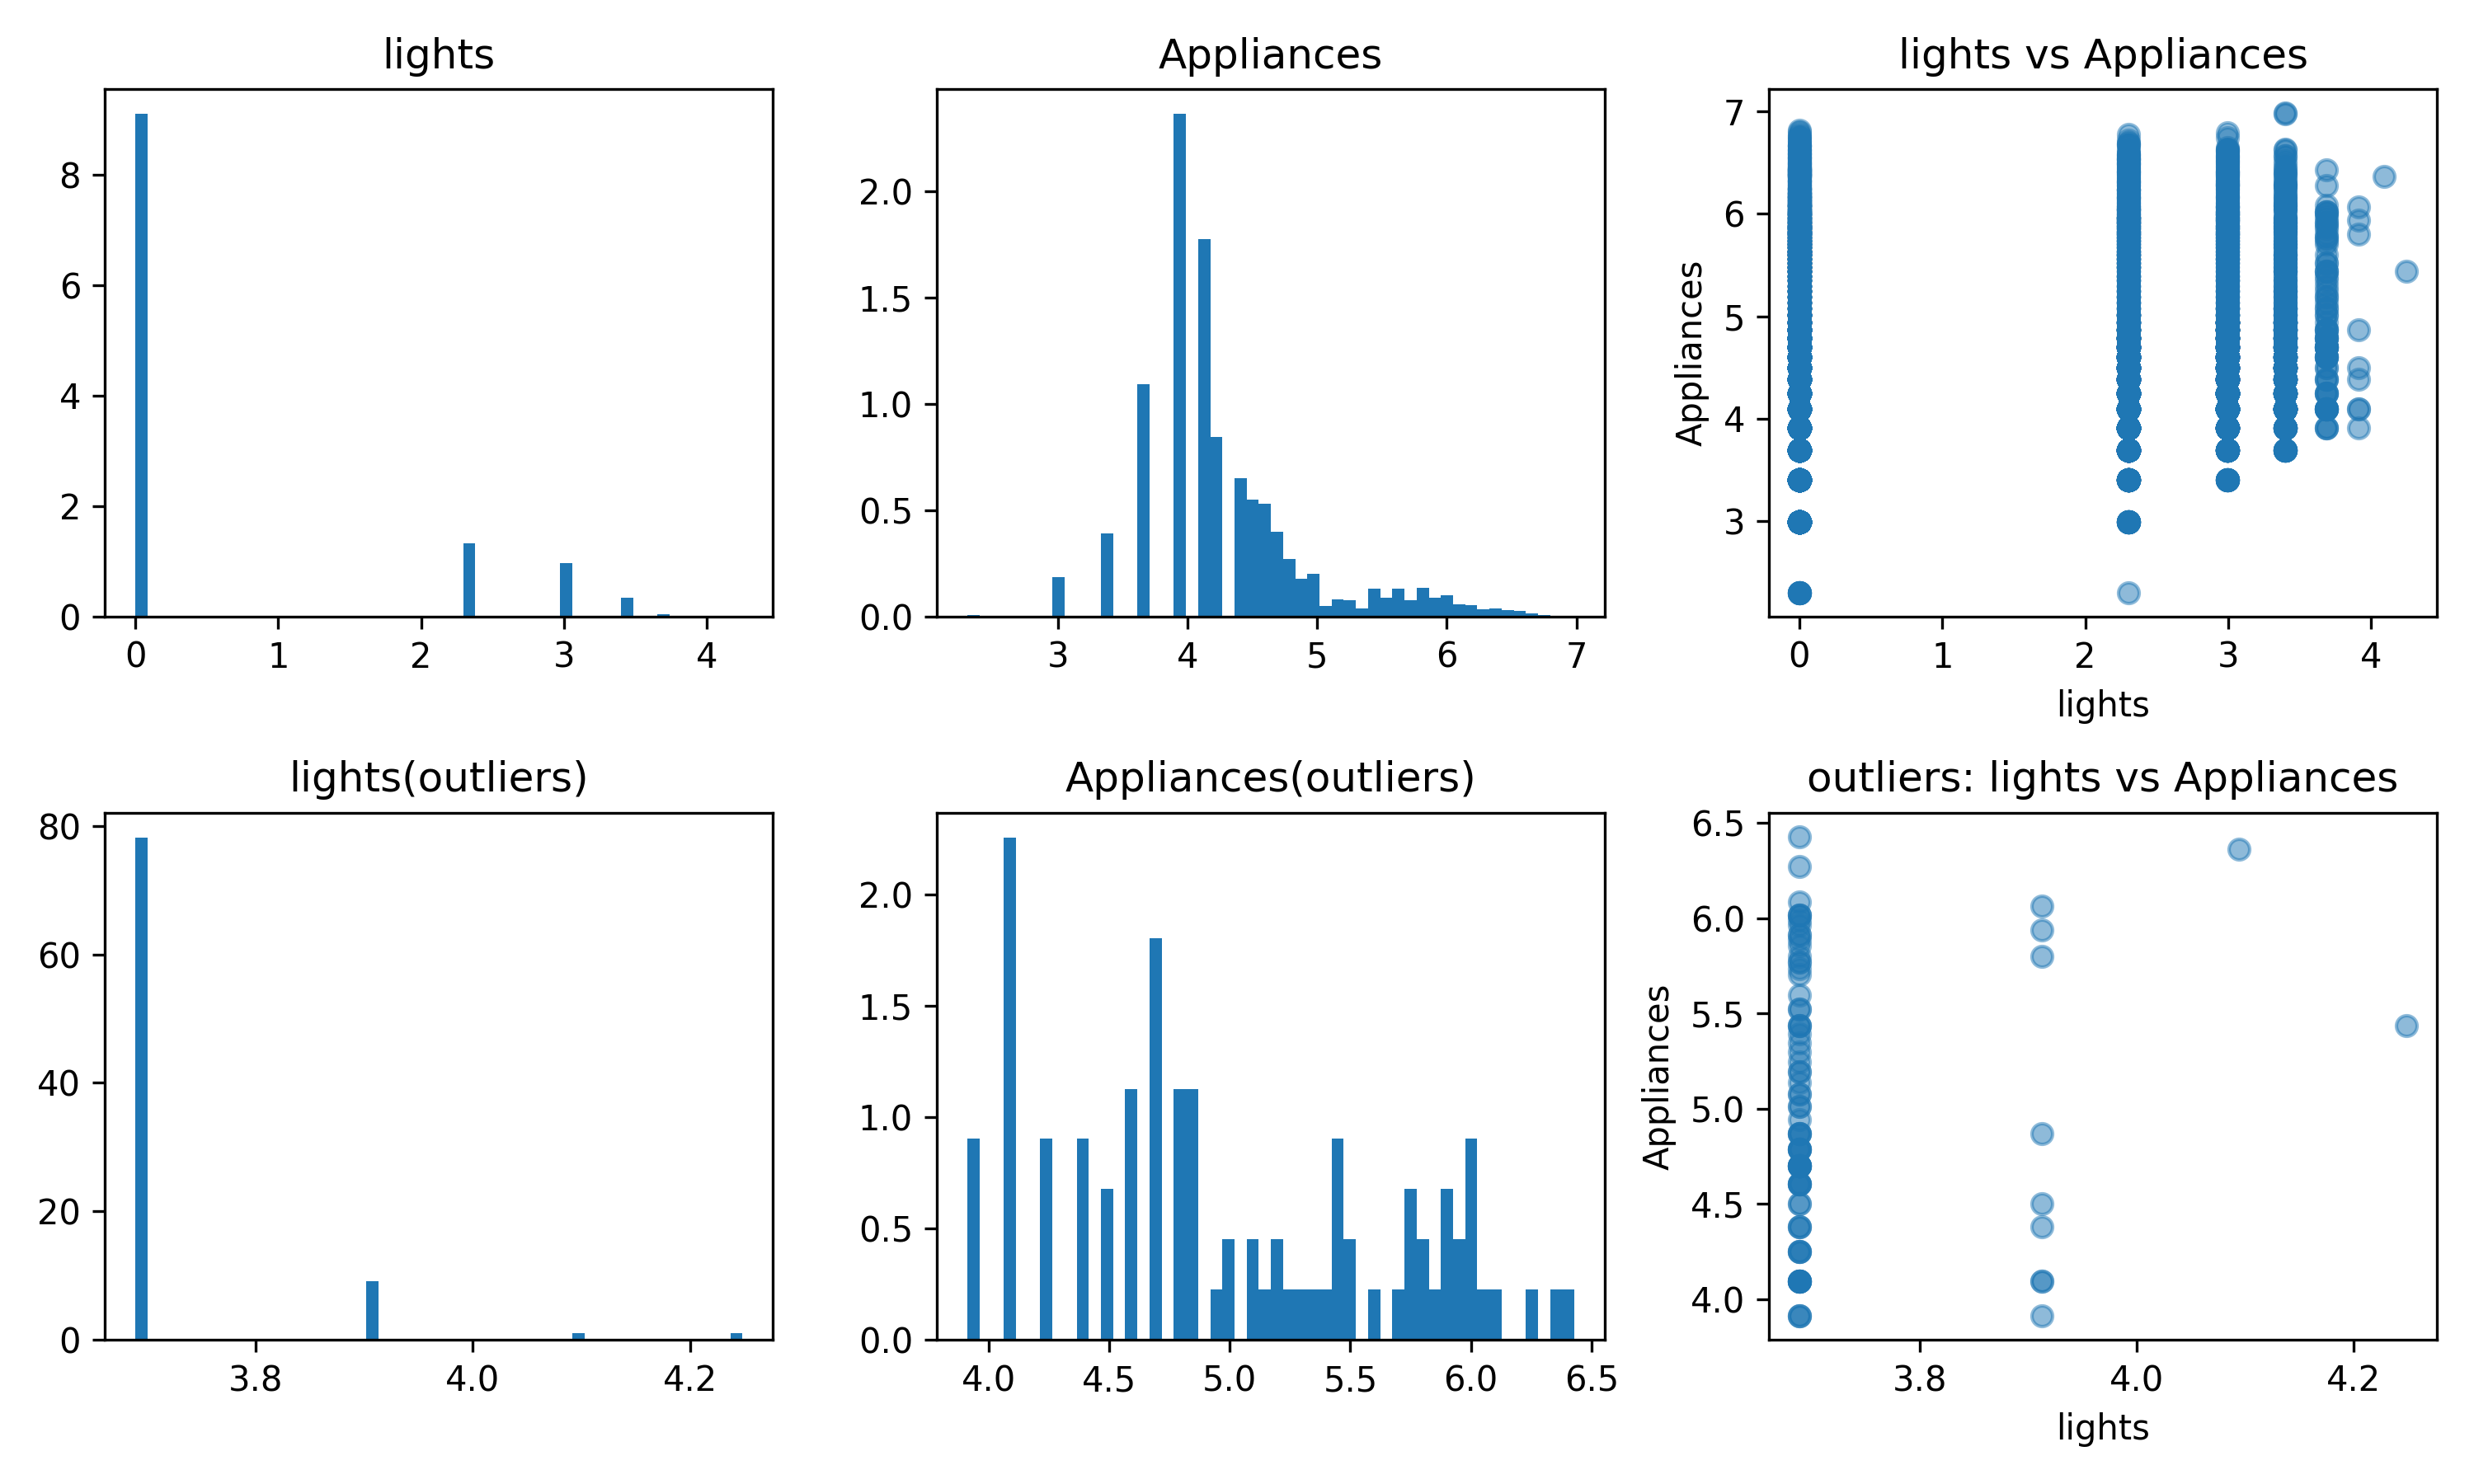
\includegraphics[width=0.9\textwidth]{../results/detect_outliers.png}
    \caption{Distribution of features before and after removing outliers}
\label{fig:skewness}
\end{figure}

\begin{figure}[!h]
    \centering
    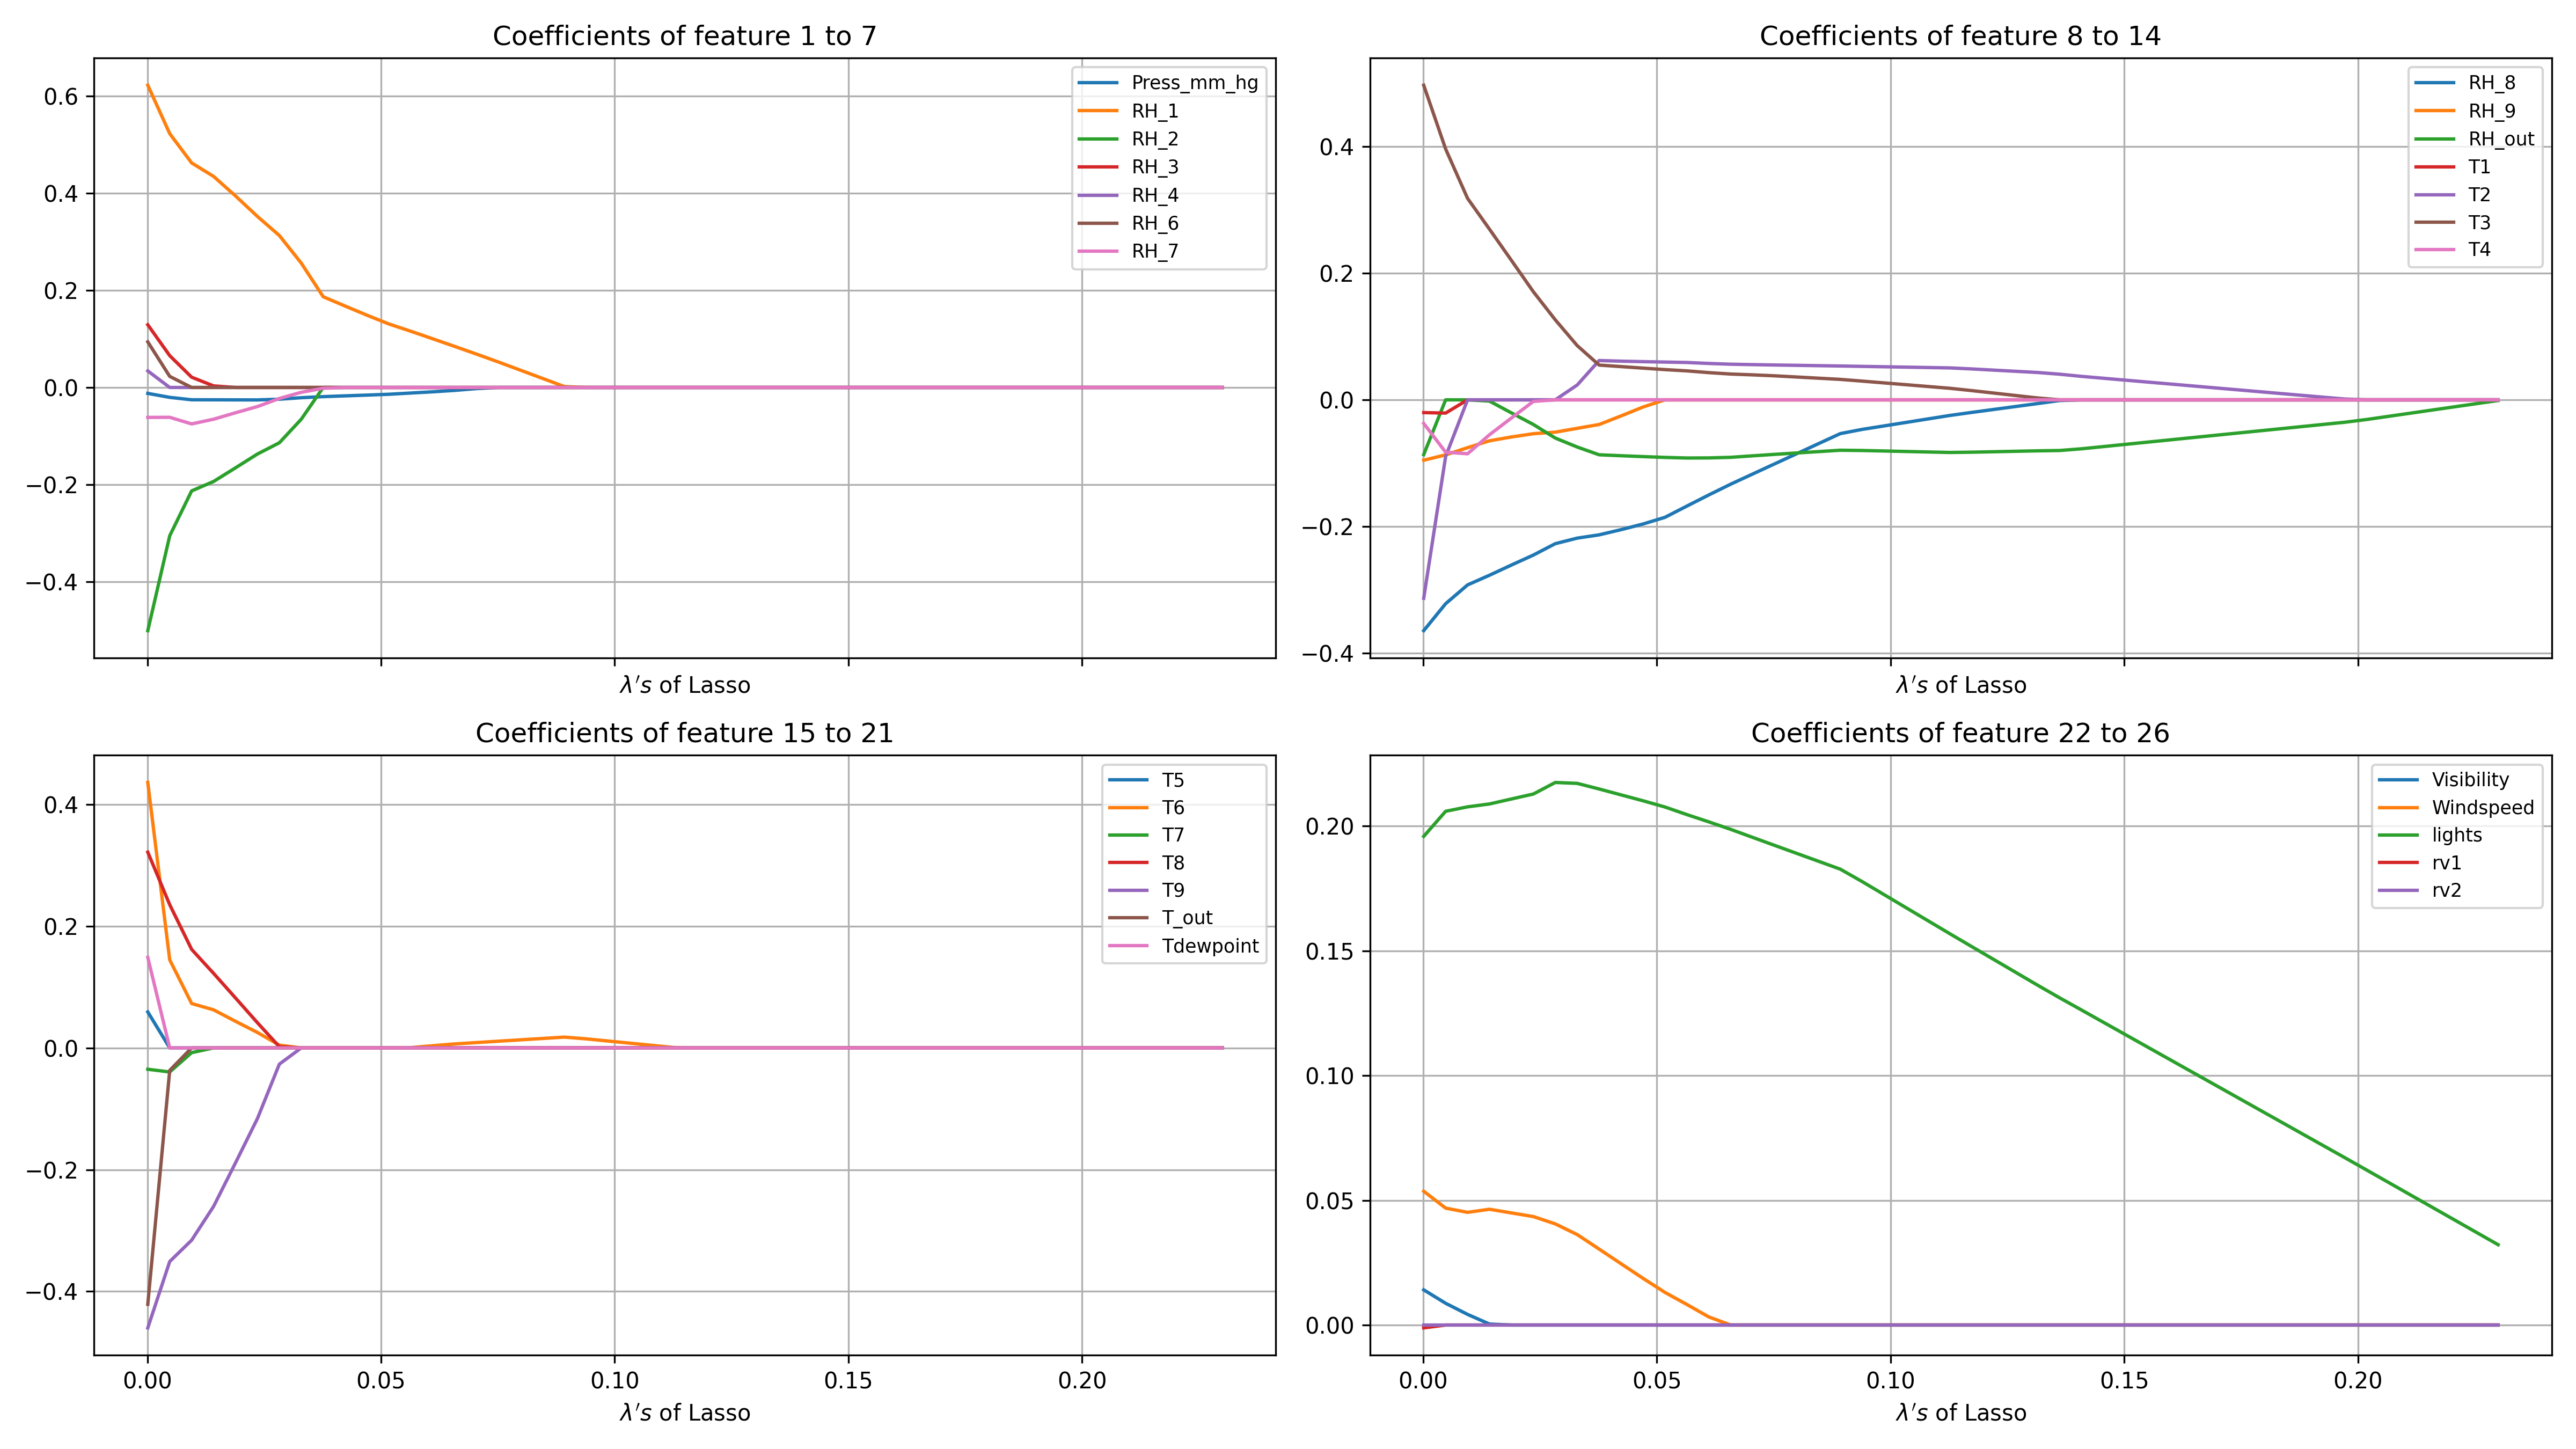
\includegraphics[width=0.9\textwidth]{../results/lasso_select.png}
    \caption{Feature selection using Lasso regression}
    \label{fig:lasso}
\end{figure}

\newpage
\subsection{Table}
\begin{center}
\begin{table}[!h]
    \centering
    \caption{OLS Regression Results}
    \label{tab:linear_regression}
    \begin{tabular}{lclc}
    \toprule
    \textbf{Dep. Variable:}    &    Appliances    & \textbf{  R-squared:         } &     0.268   \\
    \textbf{Model:}            &       OLS        & \textbf{  Adj. R-squared:    } &     0.267   \\
    \textbf{Method:}           &  Least Squares   & \textbf{  F-statistic:       } &     288.0   \\
    \textbf{Date:}             & Mon, 07 Apr 2025 & \textbf{  Prob (F-statistic):} &     0.00    \\
    \textbf{Time:}             &     03:17:47     & \textbf{  Log-Likelihood:    } &   -13165.   \\
    \textbf{No. Observations:} &       15717      & \textbf{  AIC:               } & 2.637e+04   \\
    \textbf{Df Residuals:}     &       15696      & \textbf{  BIC:               } & 2.653e+04   \\
    \textbf{Df Model:}         &          20      & \textbf{                     } &             \\
    \textbf{Covariance Type:}  &    nonrobust     & \textbf{                     } &             \\
    \bottomrule
    \end{tabular}
    \begin{tabular}{lcccccc}
                           & \textbf{coef} & \textbf{std err} & \textbf{t} & \textbf{P$> |$t$|$} & \textbf{[0.025} & \textbf{0.975]}  \\
    \midrule
    \textbf{const}         &       4.8865  &        0.595     &     8.210  &         0.000        &        3.720    &        6.053     \\
    \textbf{Press\_mm\_hg} &      -0.0021  &        0.001     &    -2.897  &         0.004        &       -0.004    &       -0.001     \\
    \textbf{RH\_1}         &       0.0861  &        0.004     &    24.388  &         0.000        &        0.079    &        0.093     \\
    \textbf{RH\_2}         &      -0.0423  &        0.003     &   -14.670  &         0.000        &       -0.048    &       -0.037     \\
    \textbf{RH\_3}         &       0.0047  &        0.004     &     1.091  &         0.275        &       -0.004    &        0.013     \\
    \textbf{RH\_7}         &      -0.0104  &        0.003     &    -4.056  &         0.000        &       -0.015    &       -0.005     \\
    \textbf{RH\_8}         &      -0.0391  &        0.002     &   -15.976  &         0.000        &       -0.044    &       -0.034     \\
    \textbf{RH\_9}         &      -0.0180  &        0.003     &    -6.682  &         0.000        &       -0.023    &       -0.013     \\
    \textbf{T3}            &       0.1480  &        0.006     &    24.182  &         0.000        &        0.136    &        0.160     \\
    \textbf{T4}            &      -0.0453  &        0.006     &    -7.724  &         0.000        &       -0.057    &       -0.034     \\
    \textbf{T6}            &       0.0113  &        0.002     &     7.277  &         0.000        &        0.008    &        0.014     \\
    \textbf{T7}            &      -0.0265  &        0.009     &    -3.067  &         0.002        &       -0.043    &       -0.010     \\
    \textbf{T8}            &       0.0802  &        0.006     &    12.812  &         0.000        &        0.068    &        0.092     \\
    \textbf{T9}            &      -0.0914  &        0.011     &    -8.077  &         0.000        &       -0.114    &       -0.069     \\
    \textbf{Visibility}    &       0.0005  &        0.000     &     1.177  &         0.239        &       -0.000    &        0.001     \\
    \textbf{Windspeed}     &       0.0076  &        0.002     &     3.468  &         0.001        &        0.003    &        0.012     \\
    \textbf{lights}        &       0.1166  &        0.004     &    27.059  &         0.000        &        0.108    &        0.125     \\
    \textbf{month\_2}      &      -0.1164  &        0.020     &    -5.679  &         0.000        &       -0.157    &       -0.076     \\
    \textbf{month\_3}      &      -0.0997  &        0.029     &    -3.489  &         0.000        &       -0.156    &       -0.044     \\
    \textbf{month\_4}      &      -0.2368  &        0.033     &    -7.149  &         0.000        &       -0.302    &       -0.172     \\
    \textbf{month\_5}      &      -0.3200  &        0.042     &    -7.574  &         0.000        &       -0.403    &       -0.237     \\
    \bottomrule
    \end{tabular}
    \begin{tabular}{lclc}
    \textbf{Omnibus:}       & 3750.717 & \textbf{  Durbin-Watson:     } &    2.003  \\
    \textbf{Prob(Omnibus):} &   0.000  & \textbf{  Jarque-Bera (JB):  } & 9389.739  \\
    \textbf{Skew:}          &   1.309  & \textbf{  Prob(JB):          } &     0.00  \\
    \textbf{Kurtosis:}      &   5.736  & \textbf{  Cond. No.          } & 1.02e+05  \\
    \bottomrule
    \end{tabular}
\end{table}
    %\caption{OLS Regression Results}
    \end{center}
    Notes: \newline
     [1] Standard Errors assume that the covariance matrix of the errors is correctly specified. \newline
     [2] The condition number is large, 1.02e+05. This might indicate that there are \newline
     strong multicollinearity or other numerical problems.

\subsection{Code}





\end{document}